\documentclass{article}
\usepackage{graphicx}
\usepackage{fancyhdr}
\usepackage{extramarks}
\usepackage{amsmath}
\usepackage{amsthm}
\usepackage{amsfonts}
\usepackage{tikz}
\usepackage[plain]{algorithm}
\usepackage{algpseudocode}
\usepackage{enumerate}
\usepackage{tikz}
\usepackage{xifthen}
\usepackage{xparse}
\usepackage{listings}
\usepackage{amsmath, amssymb}
\usepackage{subfigure}
\usepackage{lipsum}

\usetikzlibrary{automata,positioning}

%
% Basic Document Settings
%  

\topmargin=-0.45in
\evensidemargin=0in
\oddsidemargin=0in
\textwidth=6.5in
\textheight=9.0in
\headsep=0.25in

\linespread{1.1}

\pagestyle{fancy}
\lhead{\hmwkAuthorName}
\chead{\hmwkClass : \hmwkTitle}
\rhead{\firstxmark}
\lfoot{\lastxmark}
\cfoot{\thepage}

\renewcommand\headrulewidth{0.4pt}
\renewcommand\footrulewidth{0.4pt}

\setlength\parindent{0pt}

%
% Create Problem Sections
%

\newcommand{\enterProblemHeader}[1]{
    \nobreak\extramarks{}{Problem \arabic{#1} continued on next page\ldots}\nobreak{}
    \nobreak\extramarks{Problem \arabic{#1} (continued)}{Problem \arabic{#1} continued on next page\ldots}\nobreak{}
}

\newcommand{\exitProblemHeader}[1]{
    \nobreak\extramarks{Problem \arabic{#1} (continued)}{Problem \arabic{#1} continued on next page\ldots}\nobreak{}
    \stepcounter{#1}
    \nobreak\extramarks{Problem \arabic{#1}}{}\nobreak{}
}

\newcommand*\circled[1]{\tikz[baseline=(char.base)]{
		\node[shape=circle,draw,inner sep=2pt] (char) {#1};}}


\setcounter{secnumdepth}{0}
\newcounter{partCounter}
\newcounter{homeworkProblemCounter}
\setcounter{homeworkProblemCounter}{1}
\nobreak\extramarks{Problem \arabic{homeworkProblemCounter}}{}\nobreak{}

%
% Homework Problem Environment
%
% This environment takes an optional argument. When given, it will adjust the
% problem counter. This is useful for when the problems given for your
% assignment aren't sequential. See the last 3 problems of this template for an
% example.
%

\newenvironment{homeworkProblem}[1][-1]{
    \ifnum#1>0
        \setcounter{homeworkProblemCounter}{#1}
    \fi
    \section{Problem \arabic{homeworkProblemCounter}}
    \setcounter{partCounter}{1}
    \enterProblemHeader{homeworkProblemCounter}
}{
    \exitProblemHeader{homeworkProblemCounter}
}

%
% Homework Details
%   - Title
%   - Class
%   - Due date
%   - Name
%   - Student ID

\newcommand{\hmwkTitle}{Homework\ \#11}
\newcommand{\hmwkClass}{Probability \& Statistics for EECS}
\newcommand{\hmwkDueDate}{April 30, 2023}
\newcommand{\hmwkAuthorName}{Wang Yunfei}
\newcommand{\hmwkAuthorID}{2021533135}


%
% Title Page
%

\title{
    \vspace{2in}
    \textmd{\textbf{\hmwkClass:\\  \hmwkTitle}}\\
    \normalsize\vspace{0.1in}\small{Due\ on\ \hmwkDueDate\ at 23:59}\\
	\vspace{4in}
}

\author{
	Name: \textbf{\hmwkAuthorName} \\
	Student ID: \hmwkAuthorID}
\date{}

\renewcommand{\part}[1]{\textbf{\large Part \Alph{partCounter}}\stepcounter{partCounter}\\}

%
% Various Helper Commands
%

% Useful for algorithms
\newcommand{\alg}[1]{\textsc{\bfseries \footnotesize #1}}
% For derivatives
\newcommand{\deriv}[1]{\frac{\mathrm{d}}{\mathrm{d}x} (#1)}
% For partial derivatives
\newcommand{\pderiv}[2]{\frac{\partial}{\partial #1} (#2)}
% Integral dx
\newcommand{\dx}{\mathrm{d}x}
% Alias for the Solution section header
\newcommand{\solution}{\textbf{\large Solution}}
% Probability commands: Expectation, Variance, Covariance, Bias
\newcommand{\E}{\mathrm{E}}
\newcommand{\Var}{\mathrm{Var}}
\newcommand{\Cov}{\mathrm{Cov}}
\newcommand{\Bias}{\mathrm{Bias}}

\begin{document}

\maketitle

\pagebreak

\begin{homeworkProblem}[1]
\solution
\begin{enumerate}[(a)]
    \item 
    Yes, that is because $t_1X+t_2Y+t_3(X+Y)=(t_1+t_3)X+(t_2+t_3)Y$ and $X,Y$ are i.i.d. Normal distributions. And what we have known is that the sum of independent Normal distribution is also a Normal distribution. \\
    So $(t_1+t_3)X+(t_2+t_3)Y$ is normal for any constant number $t_1$,$t_2$,$t_3$.
\end{enumerate}
\begin{enumerate}[(b)]
    \item 
    No, that is because $X+Y+(SX+SY)=(1+S)X+(1+S)Y$, at the mean time $S$ is a random sign, with 0.5 probability making $(1+S)X+(1+S)Y$ be equal to 0 when $S=-1$. So from the definition of MVN, we cannot get a MVN.
\end{enumerate}
\begin{enumerate}[(c)]
    \item
    Yes, that is because $t_1SX+t_2SY=S(t_1X+t_2Y)$, from the threom mentioned in (a), we can have $(t_1X+t_2Y)\sim N(0,t_1^2+t_2^2)$.\\
    And from what we have proved in class, we can know $Z=SW$ and $Z\sim N(0,1)$ when $W\sim N(0,1)$ and S is sign random and is independent of W.\\
    So under this situation, we can let $W=\frac{(t_1X+t_2Y)}{\sqrt{t_1^2+t_2^2}}$, then $W\sim N(0,1)$, and we have known S is independent of $(X,Y)$.\\
    Therefore $Z=SW=S\frac{(t_1X+t_2Y)}{\sqrt{t_1^2+t_2^2}}$, then $\sqrt{t_1^2+t_2^2}Z=S(t_1X+t_2Y)$ and $Z\sim N(0,1)$. Finally $S(t_1X+t_2Y)\sim N(0,t_1^2+t_2^2)$.
\end{enumerate}
\end{homeworkProblem}
\newpage
\begin{homeworkProblem}[2]

\begin{enumerate}[(1)]
    \item
    Method 1 MVN\\
    $t_1(X+Y)+t_2(X-Y)=(t_1+t_2)X+(t_1+t_2)Y$, because $X,Y$ are i.i.d. Normal distribution and because the sum of the Normal distribution is also Normal. Therefore we can get it.
\end{enumerate}
\begin{enumerate}[(2)]
    \item
    Method 2 change of variables\\
    First denote $(X+Y,X-Y)=(Z,W)$, then $Z=X+Y,\ W=X-Y$.\\
    Then we can get $z=x+y,\ w=x-y$, and then $x=\frac{z+w}{2},\ y=\frac{z-w}{2}$.\\
    Therefore we can get $\frac{\partial(x,y)}{\partial(z,w)}$,
    $\begin{pmatrix}
        0.5 & 0.5\\
        0.5 & -0.5
    \end{pmatrix}$
    Then $\left\lvert \frac{\partial(x,y)}{\partial(z,w)}\right\rvert =\frac{1}{2}$.\\
    Then $f_{Z,W}(z,w)=f_{X,Y}(x,y)*\left\lvert \frac{\partial(x,y)}{\partial(z,w)}\right\rvert=\frac{1}{2}f_{X,Y}(x,y)$.\\
    Because $X,Y$ are i.i.d. Normal distribution, then we can get $f_{Z,W}(z,w)=\frac{1}{2}f_{X}(x)f_{Y}(y)=\frac{1}{2}\frac{1}{\sqrt{2\pi}}e^{-\frac{x^2}{2}}\frac{1}{\sqrt{2\pi}}e^{-\frac{y^2}{2}}=\frac{1}{4\pi}e^{-\frac{z^2}{4}}e^{-\frac{w^2}{4}}$.\\
    Obviously we can simply it as $h(z)g(w)$, so they are independent.
\end{enumerate}
\end{homeworkProblem}
\newpage
\begin{homeworkProblem}[3]
\solution
\begin{enumerate}[(a)]
    \item
    For this question we can use change of variables method too.\\
    From the picture we can have $R=\sqrt{X^2+Y^2}$ and $\Theta=arctan(\frac{Y}{X})$.\\
    Then we have $r=\sqrt{x^2+y^2}$ and $\theta=arctan(\frac{y}{x})$.\\
    Then we can $\frac{\partial(r,\theta )}{\partial(x,y)}$ more easily.
    $\begin{pmatrix}
        \frac{x}{\sqrt{x^2+y^2}}& \frac{y}{\sqrt{x^2+y^2}}\\
        \frac{-y}{x^2+y^2} & \frac{x}{x^2+y^2}
    \end{pmatrix}$
    Therefore $\left\lvert \frac{\partial(r,\theta )}{\partial(x,y)}\right\rvert =\frac{1}{\sqrt{x^2+y^2}}$.\\
    Then $f_{R,\Theta}(r,\theta)=f_{X,Y}(x,y)*\left\lvert \frac{1}{\frac{\partial(r,\theta)}{\partial(x,y)}}\right\rvert=\sqrt{x^2+y^2}f_{X,Y}(x,y)$.\\
    Because $X,Y$ are i.i.d. Normal distribution, then we can get $f_{R,\Theta}(r,\theta)=\sqrt{x^2+y^2}f_{X}(x)f_{Y}(y)=r\frac{1}{\sqrt{2\pi}}e^{-\frac{x^2}{2}}\frac{1}{\sqrt{2\pi}}e^{-\frac{y^2}{2}}$.\\
    And we have $x^2=\frac{r^2}{1+tan^2\theta}$, $y^2=\frac{r^2tan^2\theta}{1+tan^2\theta}$, then we have,\\
    $f_{R,\Theta}(r,\theta)=\frac{r}{2\pi}e^{-\frac{r^2}{2}}$.\\
    And obviously $\theta$ is distributed as Uniform distribution, so they are independent.\\
\end{enumerate}
\end{homeworkProblem}
\newpage
\begin{homeworkProblem}[4]
\solution
\begin{enumerate}[(a)]
    \item 
    For this question we can use change of variables method too.\\
    From the question we can have $T=X+Y$, $W=\frac{X}{Y}$.\\
    Then we have $t=x+y$, $w=\frac{x}{y}$.\\
    Then $x=\frac{wt}{w+1}$, $y=\frac{t}{w+1}$.\\
    Then we can $\frac{\partial(t,w )}{\partial(x,y)}$ more easily.
    $\begin{pmatrix}
        1& 1\\
        \frac{1}{y} & -\frac{x}{y^2}
    \end{pmatrix}$
    Therefore $\left\lvert \frac{\partial(t,w )}{\partial(x,y)}\right\rvert =\frac{x+y}{y^2}$.\\
    Then $f_{T,W}(t,w)=f_{X,Y}(x,y)*\left\lvert \frac{1}{\frac{\partial(t,w)}{\partial(x,y)}}\right\rvert=\frac{y^2}{x+y}f_{X,Y}(x,y)$.\\
    Because $X,Y$ are i.i.d. exponential distribution, then we can get $f_{T,W}(t,w)=\frac{y^2}{x+y}f_{X}(x)f_{Y}(y)=\frac{y^2}{x+y}\lambda e^{-\lambda x}\lambda e^{-\lambda y}$\\
    Therefore $f_{T,W}(t,w)=\frac{1}{(w+1)^2}\lambda^2te^{-\lambda t}$.\\
    Obviously it can be denoted as $h(w)g(t)$, then they are independent.\\
    Because $\int_{0}^{\infty} \frac{1}{(1+w)^2} \,dw=1$.\\
    Finally we can have $f_W(w)=\frac{1}{(1+w)^2}$, and $f_T(t)=\lambda^2te^{-\lambda t}$.
\end{enumerate}
\begin{enumerate}[(b)]
    \item 
    First let $T=X+Y$, then we can have $f_T(t)=t$ when $0<t<1$, and $f_T(t)=2-t$ when $1<t<2$, otherwise =0.\\
    Then $W=X+Y+Z=T+Z$, with $0<w-t<1$ and by using convolution method, we have,\\
    $f_W(w)=\int_{-\infty}^{+\infty}f_T(t)f_Z(w-t)  \,dt=\int_{w-1}^{w}f_T(t)*1 \,dt $.\\
    When $0<w<1$,\\
    $\int_{w-1}^{w}f_T(t) \,dt=\int_{0}^{w}t \,dt=\frac{w^2}{2}$.\\
    When $1<w<2$,\\
    $\int_{w-1}^{w}f_T(t) \,dt=\int_{w-1}^{1}t \,dt+\int_{1}^{w}2-t \,dt=-w^2+3w-\frac{3}{2}$.\\
    When $2<w<3$,\\
    $\int_{w-1}^{w}f_T(t) \,dt=\int_{w-1}^{2}2-t \,dt=\frac{(w-3)^2}{2}$.\\
    Otherwise =0.
\end{enumerate}
\begin{enumerate}[(c)]
    \item 
    method 1 convolution:\\
    $F_M(t)=P(M<=t)=P(X<=t,Y<=t)$.\\
    Because they are i.i.d. exponential distribution. \\
    Then $F_M(t)=P(X<=t)P(Y<=t)=(1-e^{-\lambda t})^2$. \\
    Then we can get $f_M(t)=2\lambda e^{-2\lambda t}*(e^{\lambda t}-1)$ by derivation.\\
    $f_{X+\frac{1}{2}Y}(t)=\int_{-\infty}^{+\infty}f_X(x)f_{\frac{1}{2}Y}(t-x) \,dx=\int_{0}^{t}\lambda e^{-\lambda x} 2\lambda e^{-2\lambda (t-x)}\,dx=2\lambda e^{-2\lambda t}\int_{0}^{t}\lambda e^{\lambda x} \,dx$.\\
    $=2\lambda e^{-2\lambda t}*(e^{\lambda t}-1)=2\lambda e^{-\lambda t}-2\lambda e^{-2\lambda t}$.\\
    Then we get it.\\
    method 2 exponential properties:\\
    Let $L=min(X,Y)$, then we can denote M as $M=L+(M-L)$, and obviously $L\sim Expo(2\lambda)$ because we have known the PDF of $M$ and $M+L=X+Y$. \\
    That is $2\lambda e^{-\lambda t}=2\lambda e^{-\lambda t}-2\lambda e^{-2\lambda t}+L$. Then $L=2\lambda e^{-2\lambda t}$.\\
    At the same time $L$ can be seen as the subject finishing the first thing. And $M-L \sim Expo(\lambda)$, can be seen as the time of the second thing being finished.\\
    Because of the property of memorylessness, then we can add them up and it is equal to $M$. Meanwhile, $X\sim Expo(\lambda)$ and $\frac{1}{2}Y\sim Expo(2\lambda)$.\\
    Therefore, we get it.

\end{enumerate}
\end{homeworkProblem}
\newpage
\begin{homeworkProblem}[5]
\solution
\begin{enumerate}[(a)]
    \item 


\begin{figure}[htbp]
    \centering
    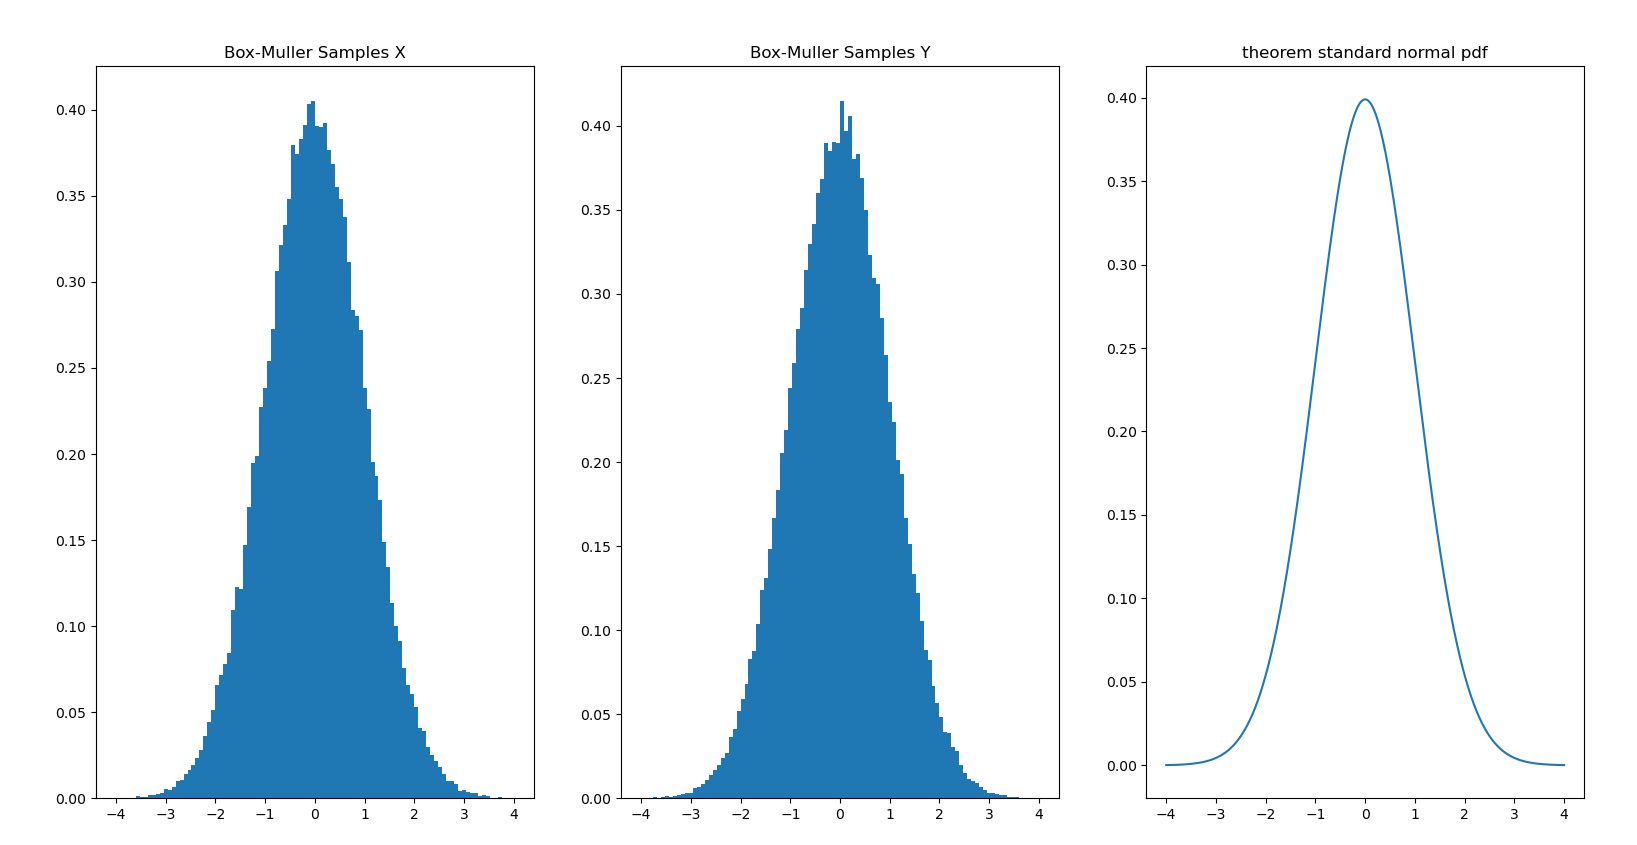
\includegraphics[width=0.5\textwidth]{0.png}
    \caption{figure 1}
    \end{figure} 


\end{enumerate}
\begin{enumerate}[(b)]
    \item
    \begin{figure}[htbp]
        \centering
        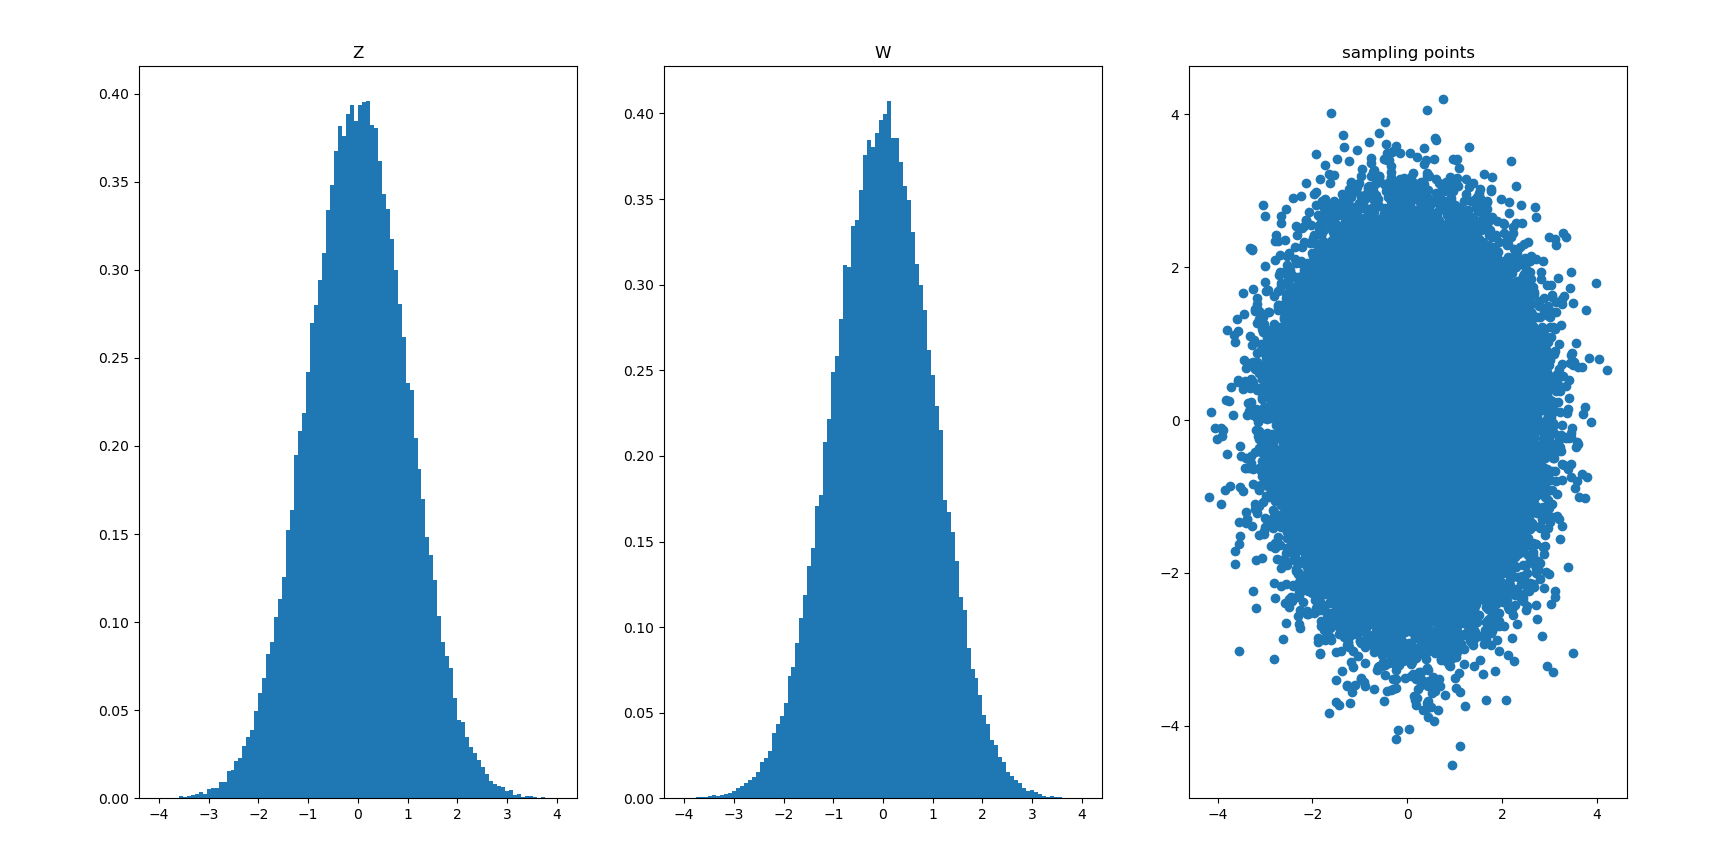
\includegraphics[width=0.5\textwidth]{1.png}
        \caption{figure 2}
        \end{figure} 
\end{enumerate}
\begin{enumerate}[(c)]
    \item
    \begin{figure}[htbp]
        \centering
        \subfigure[Fig1]{
        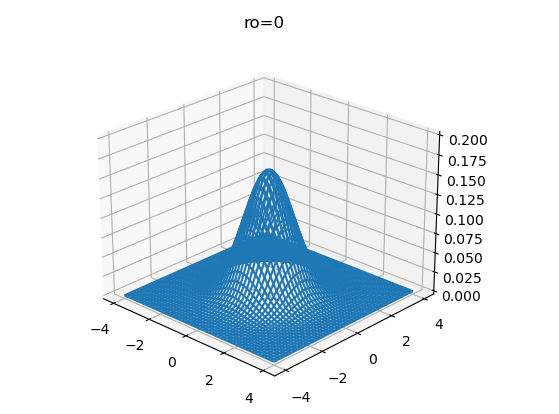
\includegraphics[scale=0.25]{sub1.png} \label{1}
        }
        \quad
        \subfigure[Fig2]{
        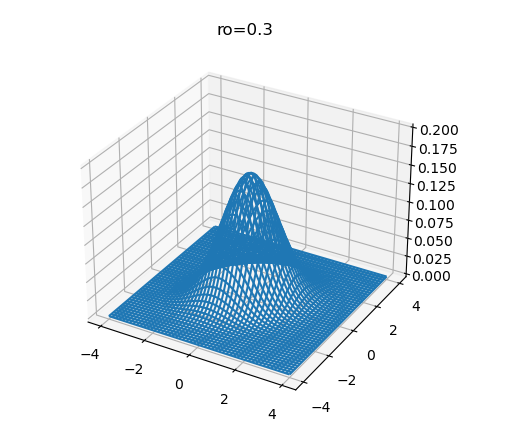
\includegraphics[scale=0.25]{sub2.png} \label{2} 
        }
        \quad
        \subfigure[Fig3]{
        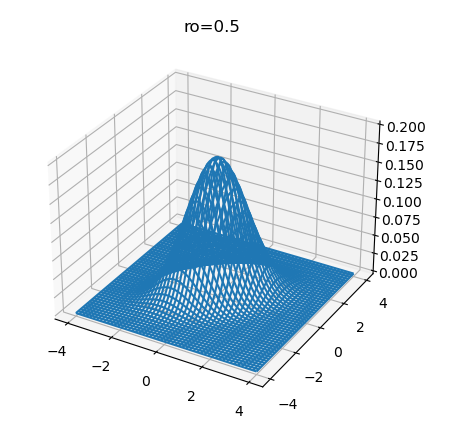
\includegraphics[scale=0.25]{sub3.png}\label{3}
        }
        \quad
        \subfigure[Fig4]{
        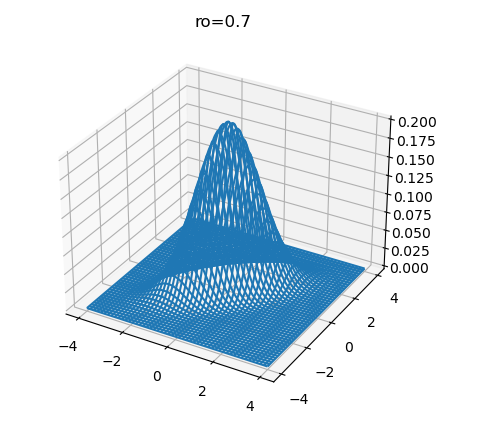
\includegraphics[scale=0.25]{sub4.png}\label{4}
        }
        \quad
        \subfigure[Fig5]{
        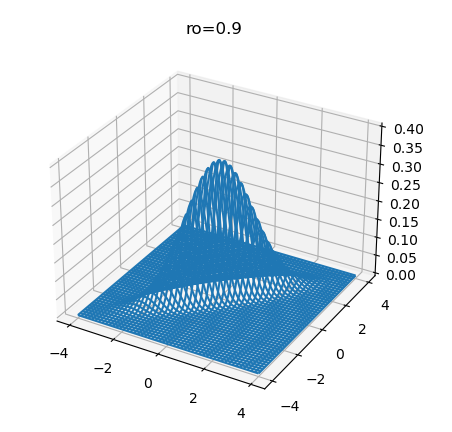
\includegraphics[scale=0.25]{sub5.png}\label{5}
        }
        \caption{figure 3 3D}
        \end{figure}
    
    \begin{figure}[htbp]
        \centering
        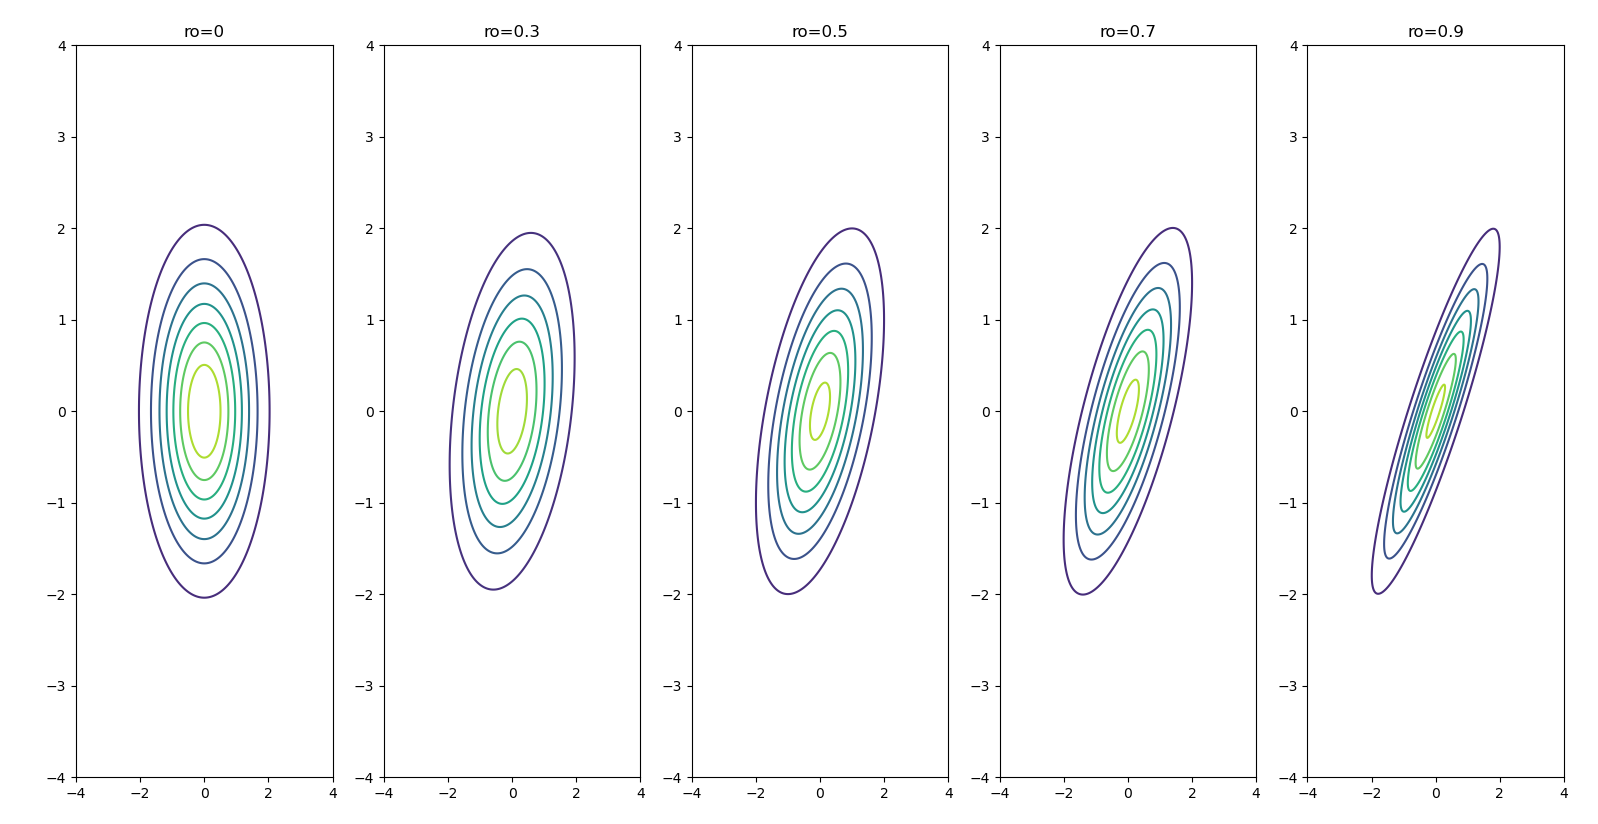
\includegraphics[width=0.6\textwidth]{2.png}
        \caption{figure 4 contour}
        \end{figure} 
\end{enumerate}
\newpage
\begin{verbatim}
    import numpy as np
    import matplotlib.pyplot as plt
    import math
    from scipy.stats import multivariate_normal
    ##(1)
    ###unif
    u1=np.random.random(100000)
    u2=np.random.random(100000)
    x1 = np.linspace(0 - 4 , 0 + 4, 1000)
    R=np.sqrt(-2*np.log(u1))
    theta=2*np.pi*u2
    x=R*np.cos(theta)
    y=R*np.sin(theta)
    theorem=(1/np.sqrt(2*np.pi))*np.exp(-(x1**2)/2)
    plt.figure(1)
    plt.subplot(1,3,1)
    plt.hist(x,bins=100,range=(-4,4),density=True)
    plt.title("Box-Muller Samples X")
    plt.subplot(1,3,2)
    plt.hist(y,bins=100,range=(-4,4),density=True)
    plt.title("Box-Muller Samples Y")
    plt.subplot(1,3,3)
    plt.title("theorem standard normal pdf")
    plt.plot(x1,theorem)
    plt.show()
    ##(2)
    ##because x y are independent so ro=0
    ro=0
    ##(Z,W) is the MVN which we have learned in class
    z=x
    w=ro*x+np.sqrt(1-ro**2)*y
    plt.figure(2)
    plt.subplot(1,3,1)
    plt.hist(z,bins=100,range=(-4,4),density=True)
    plt.title("Z")
    plt.subplot(1,3,2)
    
    plt.hist(w,bins=100,range=(-4,4),density=True)
    plt.title("W")
    plt.subplot(1,3,3)
    plt.scatter(z,w)
    plt.title("sampling points")
    plt.show()
    ##(3)
    ##set ro
    ro_vector=[0,0.3,0.5,0.7,0.9]
    ##initial other parameters
    cov=[[1,0],[0,1]]
    u=[0,0]
    x2 = np.linspace(0 - 4 , 0 + 4, 1000)
    x3 = np.linspace(0 - 4 , 0 + 4, 1000)
    Z,W=np.meshgrid(x2,x3)
    space=np.empty(Z.shape+(2,))
    space[:,:,0]=Z
    space[:,:,1]=W
    plt.figure(3)
    for i in range(5):
        ##set parameters
        ro=ro_vector[i]
        cov[1][0]=ro
        cov[0][1]=ro
        #generate mvn
        generate_mvn=multivariate_normal(u,cov)
        U=generate_mvn.pdf(space)
        plt.subplot(1,5,i+1)
        plt.contour(Z,W,U)
        plt.title(f"ro={ro}")
    plt.show()
    fig=plt.figure()
    ax=fig.add_subplot(projection='3d')
    ax.set_zlim(0,0.2)
    wframe=None
    ##set parameters
    ro=ro_vector[0]
    cov[1][0]=ro
    cov[0][1]=ro
    #generate mvn
    generate_mvn=multivariate_normal(u,cov)
    U=generate_mvn.pdf(space)
    wframe=ax.plot_wireframe(Z,W,U)
    
    plt.title(f"ro={ro}")
    plt.show()
    fig=plt.figure()
    ax=fig.add_subplot(projection='3d')
    ax.set_zlim(0,0.2)
    wframe=None
    ##set parameters
    ro=ro_vector[1]
    cov[1][0]=ro
    cov[0][1]=ro
    #generate mvn
    generate_mvn=multivariate_normal(u,cov)
    U=generate_mvn.pdf(space)
    wframe=ax.plot_wireframe(Z,W,U)
    
    plt.title(f"ro={ro}")
    plt.show()
    fig=plt.figure()
    ax=fig.add_subplot(projection='3d')
    ax.set_zlim(0,0.2)
    wframe=None
    ##set parameters
    ro=ro_vector[2]
    cov[1][0]=ro
    cov[0][1]=ro
    #generate mvn
    generate_mvn=multivariate_normal(u,cov)
    U=generate_mvn.pdf(space)
    wframe=ax.plot_wireframe(Z,W,U)
    
    plt.title(f"ro={ro}")
    plt.show()
    fig=plt.figure()
    ax=fig.add_subplot(projection='3d')
    ax.set_zlim(0,0.2)
    wframe=None
    ##set parameters
    ro=ro_vector[3]
    cov[1][0]=ro
    cov[0][1]=ro
    #generate mvn
    generate_mvn=multivariate_normal(u,cov)
    U=generate_mvn.pdf(space)
    wframe=ax.plot_wireframe(Z,W,U)
    
    plt.title(f"ro={ro}")
    plt.show()
    fig=plt.figure()
    ax=fig.add_subplot(projection='3d')
    ax.set_zlim(0,0.4)
    wframe=None
    ##set parameters
    ro=ro_vector[4]
    cov[1][0]=ro
    cov[0][1]=ro
    #generate mvn
    generate_mvn=multivariate_normal(u,cov)
    U=generate_mvn.pdf(space)
    wframe=ax.plot_wireframe(Z,W,U)    
    plt.title(f"ro={ro}")
    plt.show()  
\end{verbatim}
\end{homeworkProblem}    
\end{document}
